\tab Tag-urile in Git reprezinta o metoda eficienta de a organiza mai bine lucrul nostru. Astfel putem salva sub forba de versiuni.\\
Cu comanda \textbf{git tag -a version1.0 } am creat un tag.\\
Iar cu comanda \textbf{git show NameOfTheTag} ne afiseaza versiunile disponibile si informatii aditionale.
\begin{figure}[h]
\centering
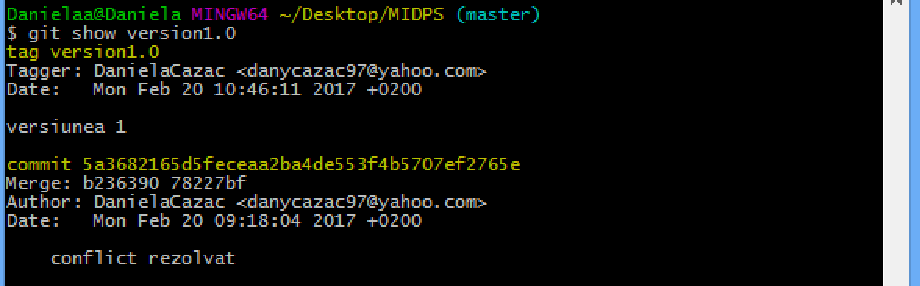
\includegraphics[scale=1]{tag.pdf}
\end{figure}

\tab Si cu comanda \textbf{git push --tags}- facem transferul tag-urilor de pe local pe site.
\begin{figure}[h]
\centering

\includegraphics[scale=1]{pushtag.pdf}
\end{figure}